\documentclass[parskip=full]{scrartcl}
\usepackage[utf8]{inputenc} % use utf8 file encoding for TeX sources
\usepackage[T1]{fontenc}    % avoid garbled Unicode text in pdf
\usepackage[german]{babel}  % german hyphenation, quotes, etc
\usepackage{hyperref}       % detailed hyperlink/pdf configuration
\hypersetup{                % ‘texdoc hyperref‘ for options
pdftitle={SWT1: Lastenheftvorlage},%
bookmarks=true,%
}

\usepackage{graphicx}       % provides commands for including figures
\usepackage{csquotes}       % provides \enquote{} macro for "quotes"
\usepackage[nonumberlist]{glossaries}     % provides glossary commands
\usepackage{enumitem}

\makenoidxglossaries
%
% % Glossareinträge
%
\newglossaryentry{Dozent}
{
	name=Dozent,
	plural=Dozenten,
	description={Leiter eines oder mehrerer Seminartypen},
}

\newglossaryentry{Kunde}
{
	name=Kunde,
	plural=Kunden,
	description={(Zahlende) Teilnehmer einer oder mehrerer Seminarveranstaltung/en}
}

\newglossaryentry{Seminartyp}
{
	name=Seminartyp,
	plural=Seminartypen,
	description={Typ einer Lehrveranstaltung (z.B. \enquote{Schöner Malen -- Anfängerkurs})}
}

\newglossaryentry{Seminarveranstaltung}
{
	name=Seminarveranstaltung,
	plural=Seminarveranstaltungen,
	description={Tatsächlich stattfindende Lehrveranstaltung (z.B. \enquote{Schöner Malen -- Anfängerkurs, Sommer 2014})}
}

\newglossaryentry{Computer}
{
	name=Computer,
	description={Gerät zur Verarbeitung zur Daten, das die Daten einlesen, verarbeiten, speichern und ausgeben kann}
}

\title{SWT1: Lastenheftvorlage}
\author{Santiago Tafur, 1854693}

\begin{document}

\maketitle

%
% % Hinweise - sollen nicht im endgültigen Dokument erscheinen, daher vor der Abgabe löschen!
%


%
% % Hier beginnt die Gliederung des Lastenhefts
%
\section{Zielbestimmung}
Die Firma Pear Corp soll durch einen Kunstfilter-App in die Lage versetzt werden, den Produkt iMage vertrieben. Die App muss eine erweitere Plug-in Architektur haben, wo es ermöglicht die Abstraktion eines Bilds durch geometrische Primitive.

\section{Produkteinsatz}
Das Produkt dient zur Kundenwaltung der Firma PearCorp. Die Kunden sollen die Möglichkeit zur Bild- Personalisierung und Bearbeitung haben.

Zielgruppe: Fotografen, Hobbyfotografen, Bildbearbeiter.

Plattform: PC mit Windows XP oder Nachfolger-Betriebssystem, Mac OS mit Captian oder Nachfolger-Betriebssystem, iOS Handy mit 9.2 oder Nachfolger-Betriebssystem und Android mit KitKat oder Nachfolger-Betriebssystem

\section{Funktionale Anforderungen}
\begin{itemize}[nosep]
\item[FA10] Abstraktion eines Bilds durch geometrische Primitive.
\item[FA20] Weitere Filter Weitere Filter sollen per In-AppKäufe erworben werden können.
\item[FA30] Kunstfilter als Plug-In modellieren.
\item[FA40] Kunden sollen das verwendete Primitiv wählen können.
\item[FA50] Vorschau des Filtereffektes für das aktuelle Bild.

\end{itemize}

\section{Produktdaten}
\begin{itemize}[nosep]
\item[PD10] Kunden In-AppKäufe zu speichern.
\item[PD20] Verschiedene Primitive Filtern zu speichern.
\item[PD30] Kunden Profiles und Daten

\end{itemize}

\section{Nichtfunktionale Anforderungen}
\begin{itemize}[nosep]
\item[NF10] Die Funktion /FA10/ muss mit den Bildformaten jpeg und png umgehen können
\item[NF20] Den Filter Prozess muss unter (1 Sekunde per 5 Iterationen) erreicht werden.
\item[NF30] Kunden können bis 10 Filter in eine Favoriten list hinfügen.
\end{itemize}

\section{Systemmodelle}

\subsection{Szenarien}

\subsection{Anwendungsfälle}
\subsubsection{Seminarorganisation}
\begin{center}
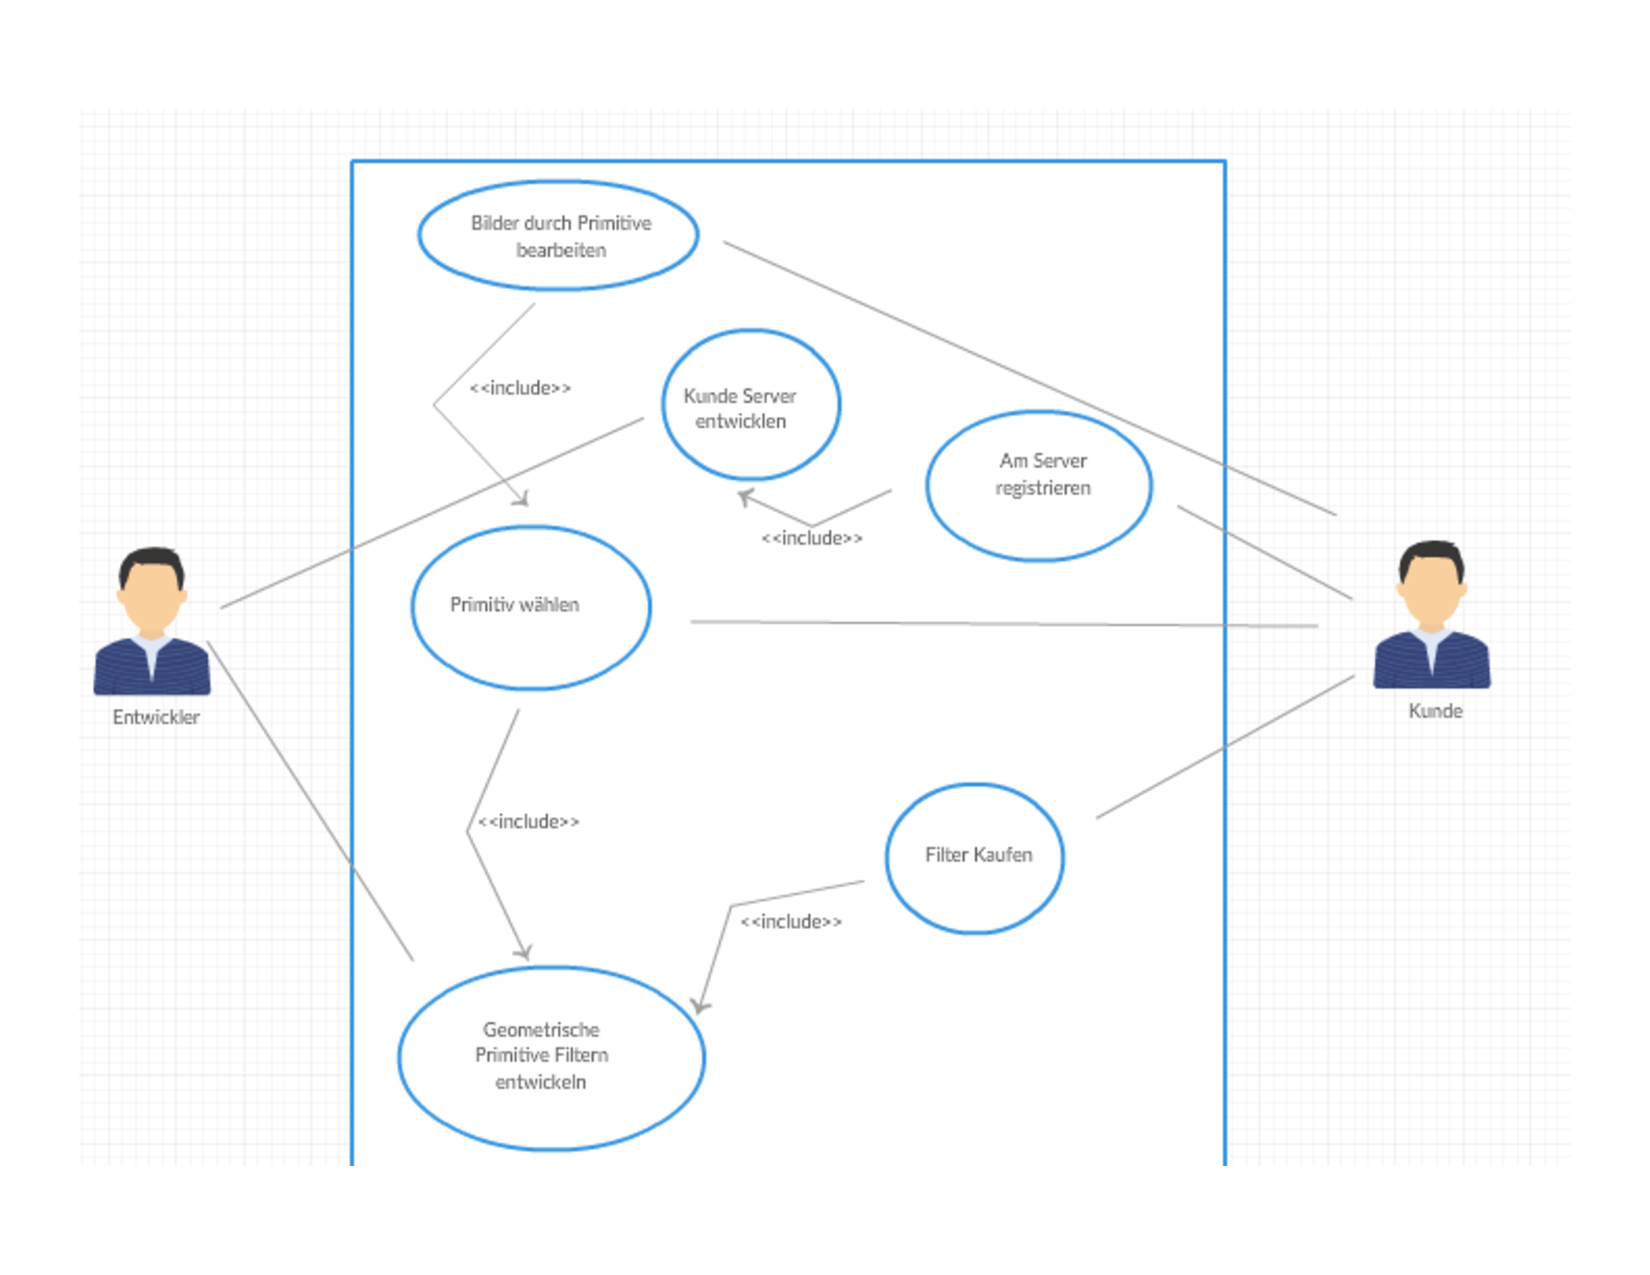
\includegraphics[width=0.8\textwidth]{szenario_seminar1.pdf}
\end{center}

Akteure: Kunde, Entwickler.

Anwendungsfälle: Bilder durch Primitive bearbeiten, Primitiv wählen, Server entwicklen, Server registrieren, Filter Kaufen, Filter entwicklen.

Textuelle Beschreibung: (folgt)



%
% % Automatisch generiertes Glossar (Latex zwei mal ausführen um Glossar anzuzeigen)
%
%\glsaddall % das sorgt dafür, dass alles Glossareinträge gedruckt werden, nicht nur die verwendeten. Das sollte nicht nötig sein!
\printnoidxglossaries





\end{document}
